\section{Theorie}
\label{sec:Theorie}

Spezielle Brückenschaltungen können Frequenzen filtern, was sie auch in der Mess- und Kommunikationstechnik wichtig macht.
Für den Grundsätzlichen Aufbau einer Brückenschaltung werden vier Widerstände benötigt.
Diese werden mit einer Speisespannung $U_\text{S}$ gespeist. Dabei werden jeweils zwei der Widerstände in Reihe geschaltet.
Diese In Reihe geschalteten Widerstandspaare werden dann wiederum parallel geschaltet wie in \ref{fig:brueckprinzip} zu sehen ist.

\begin{figure}
    \centering
    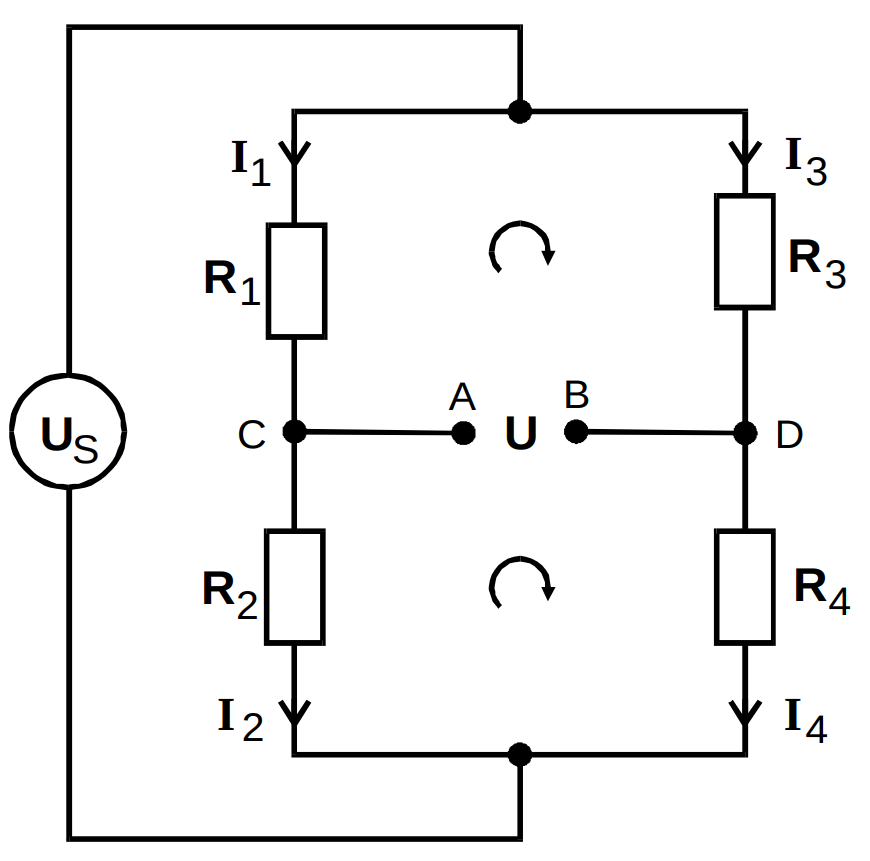
\includegraphics[scale=0.25]{content/Brueckenschaltung.png}
    \caption{Eine prinzipielle Brückenschaltung. \cite[S. 216]{anleitung}}
    \label{fig:brueckprinzip}
\end{figure}

Daraufhin lässt sich ziwschen Punkt $A$ und Punkt $B$ eine Brückspannung $U_\text{B}$ abgreifen.
Mit Hilfe der beiden Kirchhoffschen Gesetzte

\begin{enumerate}
    \item Die Summe alle zufließenden und abfließenden ströme ist gleich Null:
    
    \begin{equation}
        \sum_k I_k = 0
    \end{equation}
    \item Die Summe aller Spannungen in einer Masche nach Beachtungen der Vorzeichen ist gleich Null:
    
    \begin{equation}
        \sum_k U_k = 0
    \end{equation}
\end{enumerate}

ergibt sich dann für die Brückspannung 

\begin{equation}
    U_\text{B} = \frac{R_2\cdot R_3 - R_1 \cdot R_4}{(R_3 + R_4) \cdot (R_1 + R_2)} \cdot U_\text{S} .
    \label{eqn:Brueckspannung}
\end{equation}

Wenn nun die Widerstände $R_3$ und $R_4$ so gewählt werden, dass die Brückspannung verschwindet,
ergibt sich aus \eqref{eqn:Brueckspannung} die sogenannte Abgleichbedingung:

\begin{equation}
    R_2 R_3 = R_1 R_4 .
    \label{eqn:abgleich}
\end{equation}

\subsection{Wheatstonesche Brücke}

\begin{figure}
    \centering
    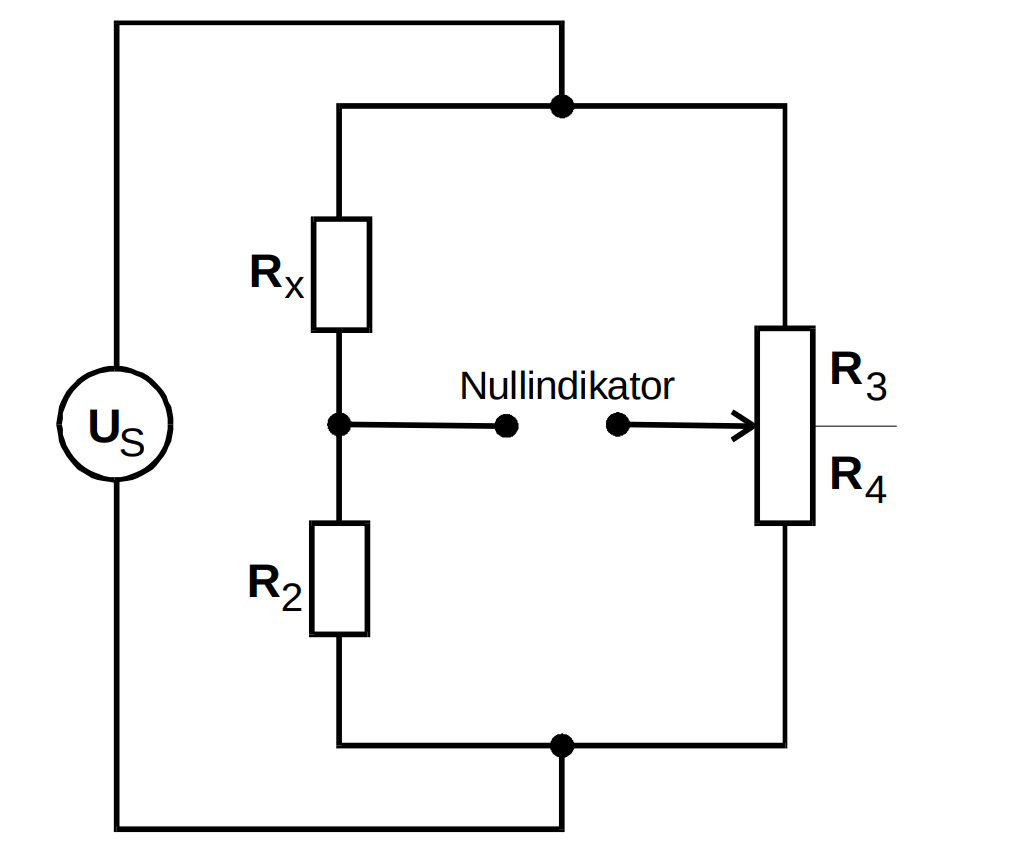
\includegraphics[scale=0.25]{content/Wheatstonesche.png}
    \caption{Die Wheatstonesche Brücke \cite[S. 219]{anleitung}.}
    \label{fig:wheatstonesche}
\end{figure}

Anstatt fester Widerstände wird nun für $R_3$ und $R_4$ ein Potentiometer verwendet.
Außerdem werden nur ohmsche Widerstände verwendet, von denen der Widerstand $R_x$ unbekannt ist.
Dieser kann ermittelt werden indem \eqref{eqn:abgleich} nach $R_x$ umgestellt wird:

\begin{equation}
    R_x = R_2 \frac{R_3}{R_4}.
    \label{eqn:abgleich_2}
\end{equation}

\subsection{Kapazitätsmessbrücke}

\begin{figure}
    \centering
    \includegraphics[scale=0.25]{content/Kapazitätsmessbruecke.png}
    \caption{Die Kapazitätsmessbrücke \cite[S. 220]{anleitung}.}
     \label{fig:kapaz}
\end{figure}

In der Kapazitätsmessbrücke sind außer ohmschen Widerständen auch Kondensatoren verbaut.
Da Kondensatoren einen Teil der elektrischen Energie in Wärme umwandeln wird ein Ersatzschaltbild genutzt.
In der Abbildung \ref{fig:kapaz} wird dies durch einen ohmschen Widerstand $R_x$ realisiert, der mit dem Kondensator $C_x$ in Reihe geschaltet ist.
Außerdem muss auch hinter den Kondensator $C_2$ mit der bekannten Kapazität ein ohmscher Widerstand $R_2$ geschaltet werden.
Dieser ist variabel um die von $R_x$ hervorgerufene Phasenverschiebung zu kompensieren.
Der unbekannte Widerstand $R_x$ kann wie in \eqref{eqn:abgleich_2} bestimmt werden.
Die Kapazität des Kondensators $C_x$ kann durch einsetzten der komplexen Widerstände in die
Abgleichbedingung \eqref{eqn:abgleich} ermittelt werden:

\begin{equation}
    C_x = C_2 \frac{R_4}{R_3}.
    \label{eqn:kapc}
\end{equation}

\subsection{Induktivitätsmessbrücke}

\begin{figure}
    \centering
    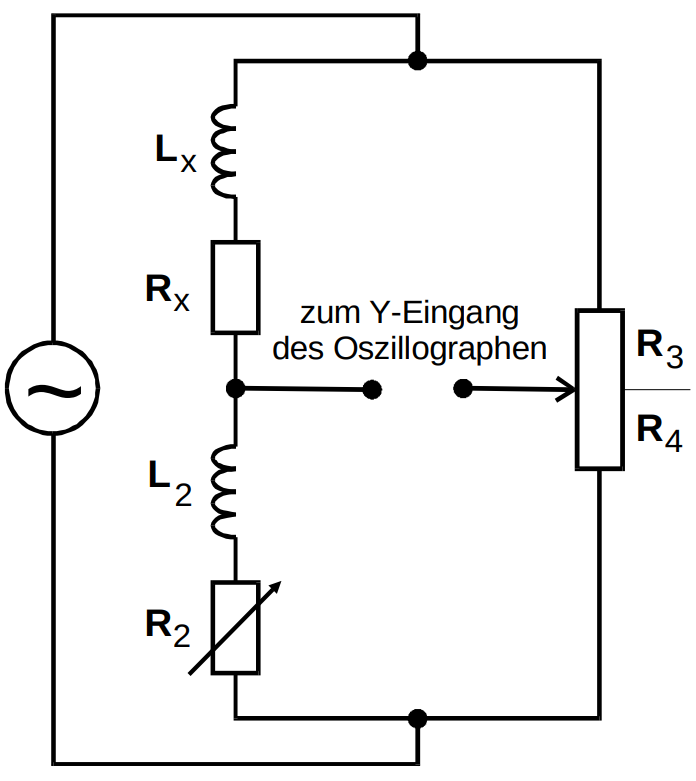
\includegraphics[scale=0.25]{content/Induktivitaetsmessbruecke.png}
    \caption{Die Induktivitätsmessbrücke \cite[S. 221]{anleitung}.}
    \label{fig:induk}
\end{figure}

Die Induktivitätsmessbrücke wird dazu genutzt unbekannte Induktivitäten zu bestimmen.
Da Spulen allerdings ähnlich wie Kondensatoren ein Teil der ihnen zugefügten elektrischen Energie in Wärme umwandeln,
wird auch für Spulen ein Ersatzschaltbild genutzt. Dieses besteht, genau wie beim Kondensaor,
aus einem ohmschen Widerstand, der mit der Spule in Reihe geschaltet wird.
Bei der Induktivitätsmessbrücke ist dies der Fall für die Spule $L_x$ mit dem ohmschen Widerstand $R_x$ (Abbildung \ref{fig:induk}).
Außerdem wird hinter die Spule $L_2$ ähnlich wie bei der Kapazitätsmessbrücke wieder ein variabler Widerstand $R_2$ gesetzt, 
um die Phasenverschiebung, die durch den Widerstand von $R_x$ auftritt, zu kompensieren.
Analog zu der Kapazitätsmessbrücke kann auch bei der Induktivitätsmessbrücke der Widerstand $R_x$ durch \eqref{eqn:abgleich_2} ermittelt werden.
Die Induktivität der Spule $L_x$ lässt sich durch

\begin{equation}
    L_x = L_2 \frac{R_3}{R_4}
    \label{eqn:indl}
\end{equation}

berechnen.

\subsection{Maxwell-Brücke}

\begin{figure}
    \centering
    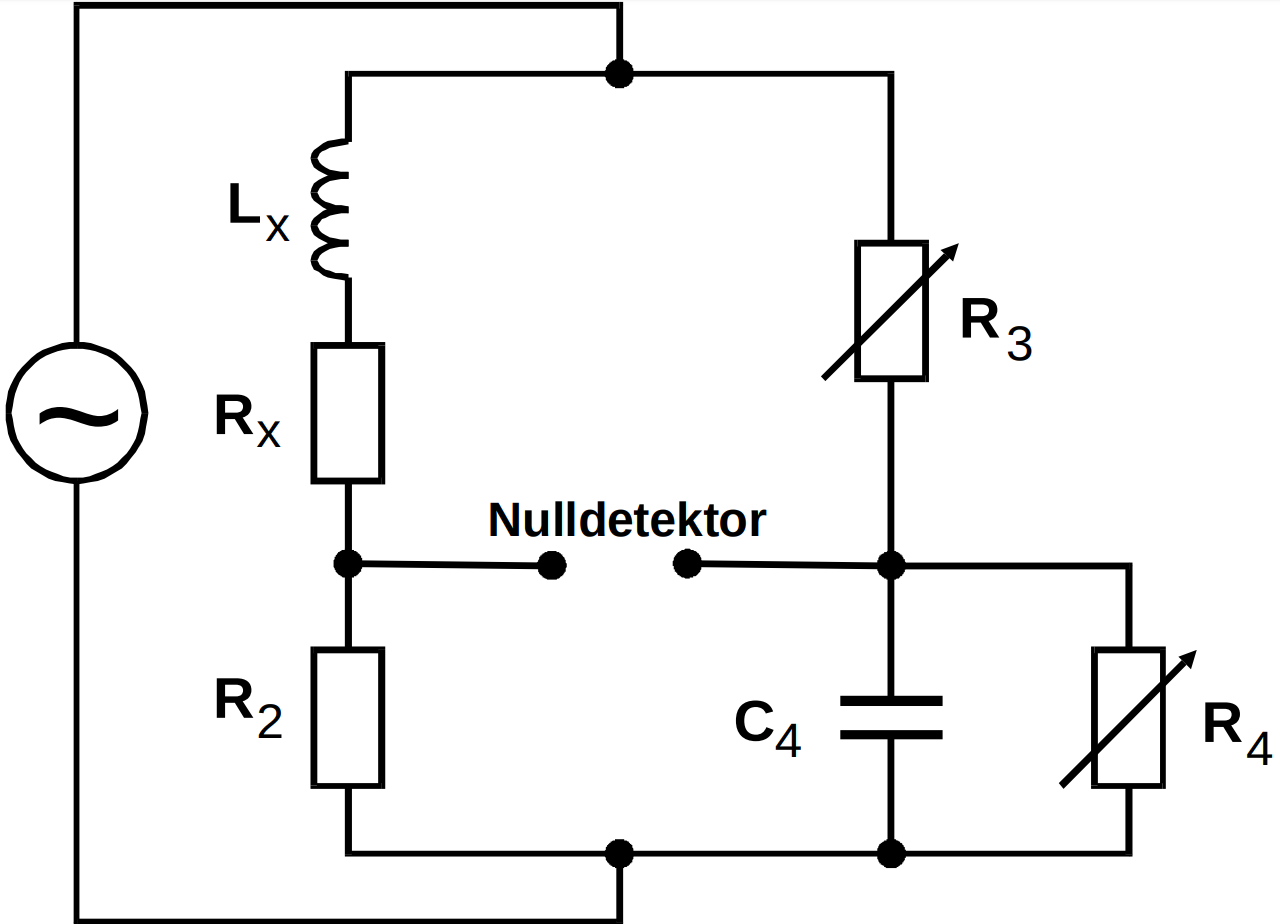
\includegraphics[scale=0.25]{content/Maxwellbruecke.png}
    \caption{Die Maxwellbrücke \cite[S. 222]{anleitung}.}
    \label{fig:maxwell}
\end{figure}

Auch mit der Maxwell-Brücke werden Induktivitäten bestimmt. 
Nun wird allerdings anstatt einer Induktivität $L_2$, eine Kapazität $C_4$ genutzt,
welche mit dem Widerstand $R_4$ parallel geschaltet wird. 
Diesmal liefert die Abgleichbedingung für den Widerstand $R_x$

\begin{equation}
    R_x = \frac{R_2 R_3}{R_4}
    \label{eqn:mw_r}
\end{equation}

und für die Induktivität $L_x$

\begin{equation}
    L_x = R_2 R_3 C_4 .
    \label{eqn:mw_l}
\end{equation}

\subsection{Wien-Robinson-Brücke}

\begin{figure}
    \centering
    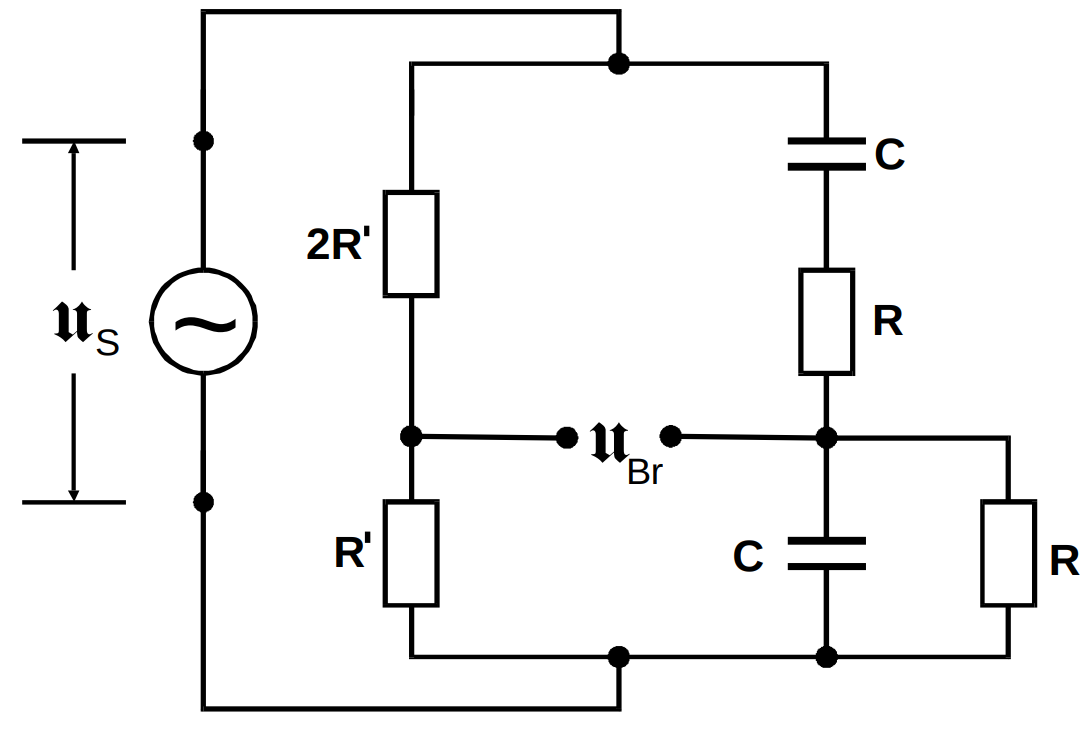
\includegraphics[scale=0.25]{content/Wien-Robinson-Bruecke.png}
    \caption{Die Wien-Robinson-Brücke \cite[S. 223]{anleitung}.}
    \label{fig:wien}
\end{figure}

In der Wien-Robinson-Brücke ist kein variabler Widerstand verbaut, wie in Abbildung \ref{fig:wien}
zu erkennen ist.
Das liegt daran, dass sie zum Filtern von Frequenzen und nicht zur Messung von Widerständen genutzt wird.
Wenn nun das Spannungsverhältnis zwischen Brücken- und Speisespannung in Abhängigkeit von der Frequenzen $\omega$ betrachtet wird 

\begin{equation}
    \left | \frac{U_B}{U_S} \right |^2 = \frac{(\omega^2R^2C^2-1)^2}{9((1-\omega^2R^2C^2) + 9 \omega^2 R^2 C^2)}
    \label{eqn:verhaeltnis}
\end{equation}

ist zu erkennen, dass die Brückspannung verschwindet, wenn 

\begin{equation}
    \omega_0 = \frac{1}{RC}
    \label{eqn:wien_rc}
\end{equation}

ist. Zur Vereinfachung wird 

\begin{equation*}
    \Omega \coloneq \frac{\omega}{\omega_0}
\end{equation*}

definiert. Damit lässt sich \eqref{eqn:verhaeltnis} umschreiben in

\begin{equation}
    \left | \frac{U_B}{U_S} \right |^2 = \frac{1}{9} \frac{(\Omega^2 -1)^2}{(1-\Omega^2)^2 + 9\Omega^2}.
    \label{eqn:wien_verh}
\end{equation}

Es fällt nun auf, dass bei der Frequenz $\omega_0$ die Brückspannung verschwinden sollte.
Dies ist allerdings in der Realität oft nicht der Fall, da Generatoren Oberwellen erzeugen.
Das Verhältnis zwischen Oberwellen und Grundwelle ist als Klirrfaktor

\begin{equation}
    k \coloneq \frac{\sqrt{\sum_{i=2} U_i^2}}{U_1}
    \label{eqn:wien_klirr}
\end{equation}

definiert. Ein idealer Generator hat den Klirrfaktor 0.